\documentclass{beamer}
\setbeamercovered{transparent}
\usetheme{Warsaw}
\usepackage[brazil,portuguese]{babel}
%\usepackage[latin1]{inputenc}
\usepackage[utf8]{inputenc}
%\usepackage[T1]{fontenc}
\usepackage{amsmath,dsfont,amsfonts,enumerate}
\usepackage{graphicx}
\usepackage{multimedia}
\newtheorem{teo}{Teorema}
\newtheorem{defi}[teo]{Defini\c{c}\~ao}
\newtheorem{demo}[teo]{Demonstra\c{c}\~ao}
\newtheorem{cor}[teo]{Corol\'ario}
\newtheorem{lem}[teo]{Lema}
\newtheorem{pro}[teo]{Proposi\c{c}\~ao}
\newtheorem{axi}[teo]{Axioma}
\newtheorem{exe}{Exemplo}
\newtheorem{exer}{Exerc\'icio}
\newtheorem{exers}{Exerc\'icios}
\newtheorem{prop}{Propriedade}
\newtheorem{nota}[teo]{Nota\c c\~ao}
\renewcommand{\leq}{\leqslant}
\renewcommand{\geq}{\geqslant}
\DeclareMathOperator*{\sen}{sen}
\DeclareMathOperator*{\tg}{tg}
\DeclareMathOperator*{\cotg}{cotg}
\DeclareMathOperator{\cossec}{cossec}
\DeclareMathOperator{\cosec}{cossec}
\DeclareMathOperator*{\senh}{senh}
\DeclareMathOperator*{\arctg}{arctg}
\newcommand{\F}{\mathds{F}}
\newcommand{\N}{\mathds{N}}
\newcommand{\Z}{\mathds{Z}}
\newcommand{\R}{\mathds{R}}
\newcommand{\Q}{\mathds{Q}}
\newcommand{\C}{\mathds{C}}
\title{Construções com régua e compasso}
\author{Nelson Alexandre Vieira Ramalho}
\institute{Universidade Federal do Amazonas - 2020}
\date{28 de setembro de 2020}
\setlength{\unitlength}{1mm}

\begin{document}


\begin{frame}
		\titlepage
\end{frame}

\section{Segmentos construtíveis}

\begin{frame}

	\frametitle{Operações fundamentais}

	As operações que podem ser feitas com esses instrumentos são chamadas de construções fundamentais; elas são: $\newline$

(1) Dados 2 pontos, podemos traçar uma linha através deles, estendendo-o indefinidamente em cada direção. $\newline$
$\newline$
(2) Dados 2 pontos, podemos traçar o segmento de linha conectando-os.$\newline$
$\newline$
(3) Dado um ponto e um segmento, podemos traçar um círculo com centro no ponto e de raio igual ao comprimento do segmento.$\newline$

\end{frame}

\begin{frame}
	Para trabalharmos com estes instrumentos, vamos definir um conjunto inicial, e a partir desse conjunto podemos obter novos pontos construtíveis. Tal conjunto deve conter pelo menos dois pontos distintos. Sendo $P_0 = \{(0,0), (1,0)\}$ o conjunto inicial para prosseguirmos com as construções. $\newline$
	$\newline$
	\begin{defi}
	Seja $P \subset \mathbb{R}^2$, contendo pelo menos dois pontos distintos, dizemos que uma reta é construtível em $P$ se dois pontos de $P$ pertencem a reta. E uma circunferência é construtível em $P$ se o centro e um ponto da circunferência estão em $P$.
	\end{defi}
\end{frame}

\begin{frame}

Tendo isso em vista, podemos obter novos pontos a partir das operações elementares:$\newline$

(I) Interseção de duas retas construídas.$\newline$

(II) Interseção de uma reta construída e uma circunferência construída.$\newline$

(III) Interseção de 2 duas circunferências construídas.$\newline$
\end{frame}

\begin{frame}
	Para trabalharmos com estes instrumentos, vamos definir um conjunto inicial, e a partir desse conjunto podemos obter novos pontos construtíveis. Tal conjunto deve conter pelo menos dois pontos distintos. Sendo $P_0 = \{(0,0), (1,0)\}$ o conjunto inicial para prosseguirmos com as construções.
\end{frame}

\begin{frame}
	Definição: Um ponto é construtível se é possível determina-lo a partir de um sequencia finita das operações elementares.$\newline$
$\newline$
Exemplo: Se $P = P_0 = \{(0, 0), (0, 1)\}$, então, como na figura abaixo, os pontos $A_1$, $A_2$, $A_3$ e $A_4$ são construtíveis em $P$, onde $A_1=(-1, 0)$, $A_2=(2, 0)$, $A_3 = (\frac{1}{2}, \frac{\sqrt3}{2})$ e $A_4 = (\frac{1}{2}, -\frac{\sqrt3}{2})$.

\end{frame}

\begin{frame}

	Lema 1: Dados um segmento de tamanho $1$ (unitário), $a$ e $b$, é possível construir os segmentos de tamanhos:$\newline$

1) $a+b$ e $a-b$, quando $a>b$. $\newline$

2) $a \cdot b$. $\newline$

3) $\dfrac{a}{b}$, quando $b \neq 0$. $\newline$
\end{frame}

\begin{frame}
	\begin{demo}
1) Sejam $O$, $A$ e $B$ pontos na reta $r$, tal que $\overline{OA} = a$ e $\overline{OB} = b$ .Traçando uma circunferência com centro em $A$ e de raio $b$, obteremos dois ponto de interseção da circunferência com a reta $r$, chamaremos de ponto $C$ o ponto à esquerda de $A$ e chamaremos de ponto $D$ o ponto à direita de A. O segmento $\overline{OD}$ tem tamanho $a + b$ e o segmento $\overline{OC}$ tem tamanho $a-b$.
\end{demo}
	\begin{figure}[h]


	\centering % para centralizarmos a figura
	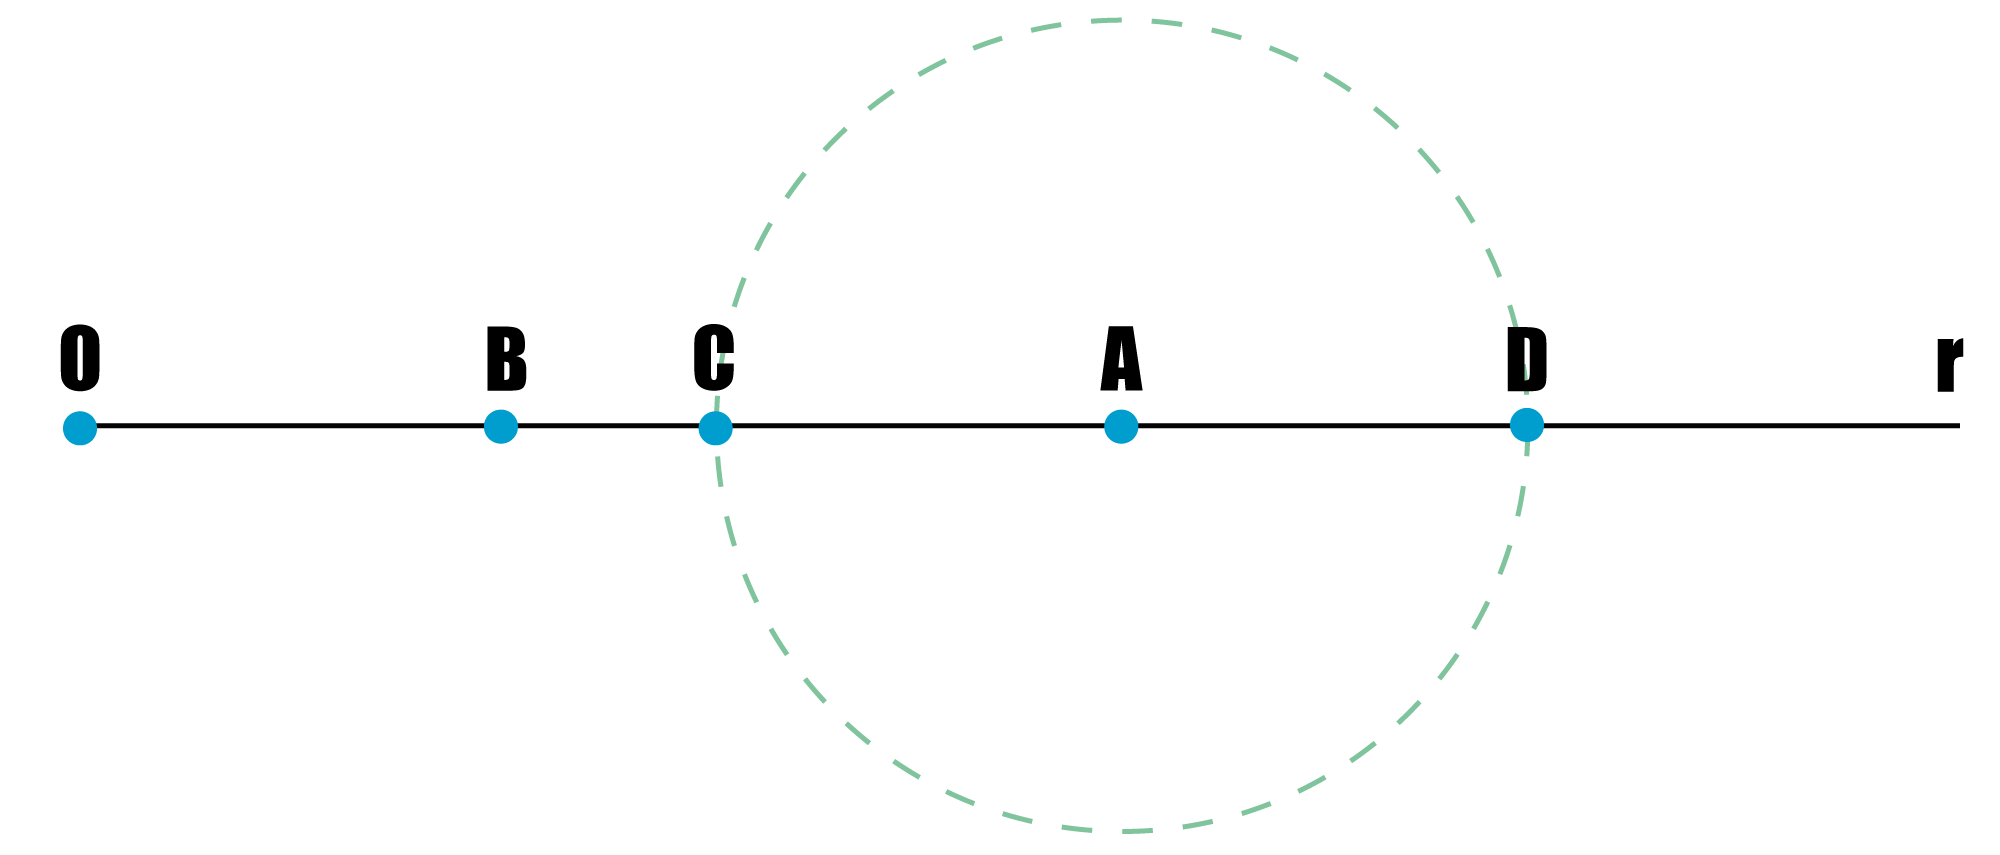
\includegraphics[height=4cm]{images/fig_6.png} % leia abaixo

	\end{figure}

\end{frame}

\begin{frame}
	\begin{demo}
	2) Sejam $O$, $U$, $A$ e $B$ pontos no plano, como na figura abaixo, tal que, $\overline{OU} = 1$, $\overline{OA} = a$, $\overline{OB} = b$. Traçando o segmento $\overline{UB}$, obtemos um triângulo $UOB$. A partir de A, traçamos uma segmento paralelo ao segmento $\overline{UB}$, a interseção desse novo segmento com o eixo $x$, chamaremos de ponto  $\overline{AB}$. Pela semelhança de triângulos:

	$\dfrac{a}{1} = \dfrac{\overline{OAB}}{b}$
$\newline$
	organizando, temos: $\overline{OAB} = a \cdot b$
\end{demo}
	\begin{figure}[h]


	\centering % para centralizarmos a figura
	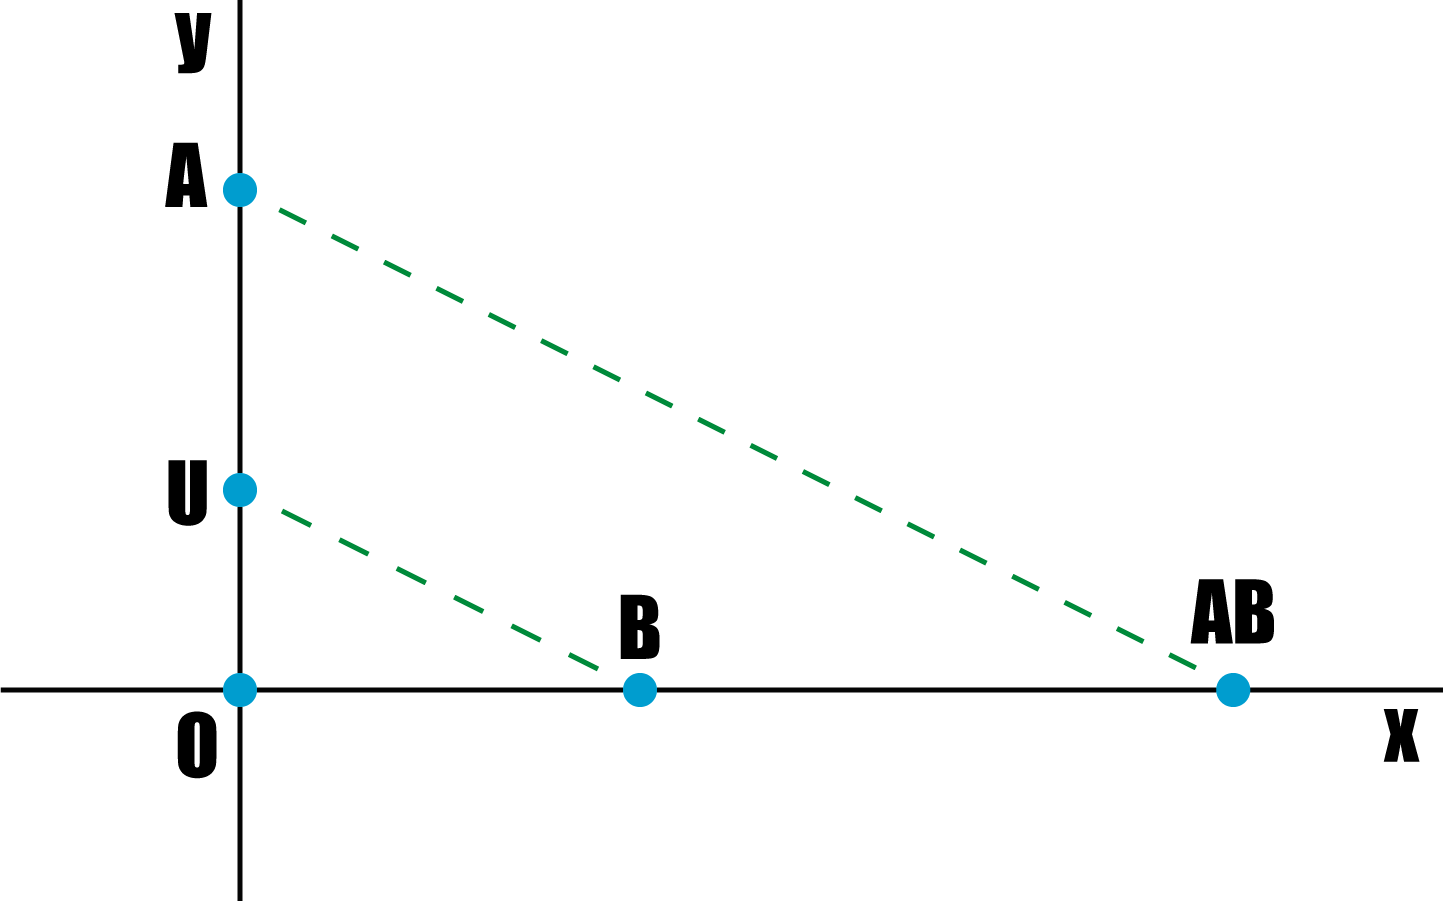
\includegraphics[height=3cm]{images/fig_7.png} % leia abaixo

	\end{figure}
\end{frame}

\begin{frame}
\begin{demo}
3) Sejam $O$, $U$, $A$ e $B$ pontos no plano, como na figura abaixo, tal que, $\overline{OU} = 1$, $\overline{OA} = a$, $\overline{OB} = b$. Traçando o segmento $\overline{AB}$, obtemos um triângulo $AOB$. A partir o ponto U, traçamos um segmento paralelo ao segmento AB, a interseção desse novo segmento com o eixo $y$, chamaremos de ponto $C$. Pela semelhança de triângulos:

$\dfrac{1}{b} = \dfrac{\overline{OC}}{a}$
$\newline$
organizando, temos:
$\overline{OC} = \dfrac{a}{b}$
\end{demo}
\begin{figure}[h]


\centering % para centralizarmos a figura
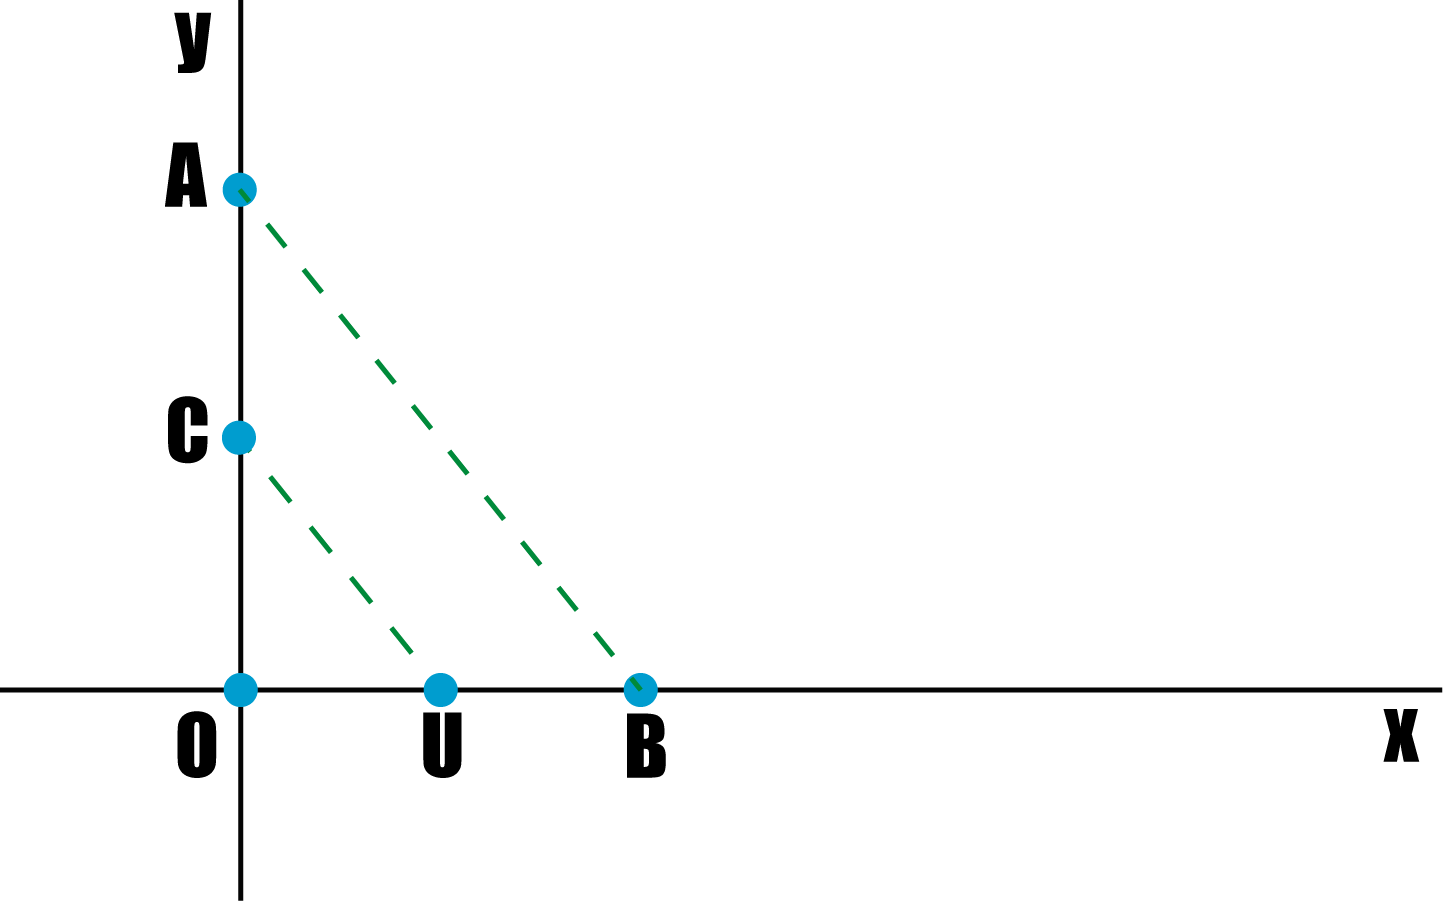
\includegraphics[height=3cm]{images/fig_8.png} % leia abaixo

\end{figure}
\end{frame}

\begin{frame}

\end{frame}
\section{Refer{\^e}ncias}

\begin{frame}

		\frametitle{Refer{\^e}ncias}
		\bibliographystyle{plain}
		\bibliography{bibliografia}
		\nocite{Gon:IA:79}
		$\newline$
		Charles Robert Hadlock.$\newline$
		Field theory and its classical problems.$\newline$
		Cambridge University Press, 2000.$\newline$

\end{frame}

\end{document}
